
%(BEGIN_QUESTION)
% Copyright 2014, Tony R. Kuphaldt, released under the Creative Commons Attribution License (v 1.0)
% This means you may do almost anything with this work of mine, so long as you give me proper credit

Suppose a voltmeter registers 0 volts between test points {\bf E} and {\bf F} in this step-down transformer circuit:

$$\includegraphics[width=15.5cm]{i03245x01.eps}$$

First, calculate the AC voltage and current we would expect to see at the load resistor.  Then, identify the likelihood of each specified fault for this circuit.  Consider each fault one at a time (i.e. no coincidental faults), determining whether or not each fault could independently account for {\it all} measurements and symptoms in this circuit.

% No blank lines allowed between lines of an \halign structure!
% I use comments (%) instead, so that TeX doesn't choke.

$$\vbox{\offinterlineskip
\halign{\strut
\vrule \quad\hfil # \ \hfil & 
\vrule \quad\hfil # \ \hfil & 
\vrule \quad\hfil # \ \hfil \vrule \cr
\noalign{\hrule}
%
% First row
{\bf Fault} & {\bf Possible} & {\bf Impossible} \cr
%
\noalign{\hrule}
%
% Another row
Fuse F1 blown &  &  \cr
%
\noalign{\hrule}
%
% Another row
Fuse F2 blown &  &  \cr
%
\noalign{\hrule}
%
% Another row
Primary windings failed open &  &  \cr
%
\noalign{\hrule}
%
% Another row
Secondary winding failed open &  &  \cr
%
\noalign{\hrule}
%
% Another row
$R_{load}$ failed shorted &  &  \cr
%
\noalign{\hrule}
%
% Another row
$R_{load}$ failed open &  &  \cr
%
\noalign{\hrule}
%
% Another row
Wire between F and H failed open &  &  \cr
%
\noalign{\hrule}
} % End of \halign 
}$$ % End of \vbox

Finally, identify the {\it next} diagnostic test or measurement you would make on this system.  Explain how the result(s) of this next test or measurement help further identify the location and/or nature of the fault.

\vfil 

\underbar{file i03245}
\eject
%(END_QUESTION)





%(BEGIN_ANSWER)

This is a graded question -- no answers or hints given!
 
%(END_ANSWER)





%(BEGIN_NOTES)

$V_{load}$ = 14.77 volts \hskip 30pt $I_{load}$ = 98.46 mA

\vskip 10pt

The lack of voltage between points E and F tells us there is no power output by the transformer.  This could be the result of a failed transformer, or something preventing power from reaching the transformer's primary winding.  Failed-open windings (either primary or secondary) are possible, as is a blown fuse F1:

% No blank lines allowed between lines of an \halign structure!
% I use comments (%) instead, so that TeX doesn't choke.

$$\vbox{\offinterlineskip
\halign{\strut
\vrule \quad\hfil # \ \hfil & 
\vrule \quad\hfil # \ \hfil & 
\vrule \quad\hfil # \ \hfil \vrule \cr
\noalign{\hrule}
%
% First row
{\bf Fault} & {\bf Possible} & {\bf Impossible} \cr
%
\noalign{\hrule}
%
% Another row
Fuse F1 blown & $\surd$ &  \cr
%
\noalign{\hrule}
%
% Another row
Fuse F2 blown &  & $\surd$ \cr
%
\noalign{\hrule}
%
% Another row
Primary windings failed open & $\surd$ &  \cr
%
\noalign{\hrule}
%
% Another row
Secondary winding failed open & $\surd$ &  \cr
%
\noalign{\hrule}
%
% Another row
$R_{load}$ failed shorted & $\surd$ & $\surd$ \cr
%
\noalign{\hrule}
%
% Another row
$R_{load}$ failed open &  & $\surd$ \cr
%
\noalign{\hrule}
%
% Another row
Wire between F and H failed open &  & $\surd$ \cr
%
\noalign{\hrule}
} % End of \halign 
}$$ % End of \vbox

Note: the fault of $R_{load}$ failed shorted is legitimate in the context of this troubleshooting question even if it causes one or both of the fuses to subsequently blow.  Some students balk at the idea of considering a shorted load as possible because that would lead to secondary faults, which they believe would violate the ``no coincidental faults'' rule.

However, it must be remembered that the rationale for the ``no coincidental faults'' rule is {\it Occam's Razor}: the principle that it is less probable for multiple, {\it coincidental} faults to occur than it is for a single fault to occur.  Since blown fuses are {\it consequent} to a shorted load, not {\it coincidental} to a shorted load, it is fair to consider a shorted load as a ``single'' (initial) fault for troubleshooting purposes even though it would lead to multiple faults when all the dust has settled.

The reason both ``possible'' and ``impossible'' cells are checked for a shorted load in this table is because one could also argue against it on the basis that fuse F2 should blow before fuse F1, in which case a shorted load could {\it not} interrupt power flow {\it to} the transformer.  This argument would be based on the observation that fuse F2 should blow at 2.5$\times$ the current value of fuse F1, but that the transformer's current step-up ratio exceeds 3:1.  However, it is truly difficult to assess which fuse would blow in a shorted-load condition without knowing a lot more about the nature of each fuse (particularily its current-time curve) and the transformer's impedance, and so either answer would be acceptable.

\vskip 10pt

A good ``next test'' would be to measure voltage at the primary winding, to see if power is even getting to there.  If so, the problem is either an open primary winding or an open secondary winding.

%INDEX% Electronics review: AC transformer circuit
%INDEX% Troubleshooting review: electric circuits

%(END_NOTES)


